\documentclass{article}
\usepackage{amsmath}
\usepackage{hyperref}
\usepackage{graphicx}
\graphicspath{{./figures/}}

\newcommand{\w}{{\mathbf w}}
\newcommand{\x}{{\mathbf x}}
\author{Thomas Hofmann, ETH Zurich \\ Andreas Tschofen, 1plusX AG}
\title{CTI Project: Deep Networks as a Semantic Platform for Modeling User Behavior Data\\ [2mm] Report: Final Results}

\begin{document}
\maketitle

\section{Changes to Milestone 3+4} 

As requested in the last intermediate report, there has been a proliferation of general platforms for deep learning and specific libraries for learning embeddings. Platforms like TensorFlow\footnote{\url{https://www.tensorflow.org/}} (Google) have become very popular and a \textit{de facto} standard in research, but also in many industries, including digital marketing (most relevant for 1plusX). The Gensim library\footnote{https://pypi.org/project/gensim/} is very popular in the area of language/text understanding and includes very efficient implementations of embedding algorithms. We have thus decided to build the required functionality on top of these frameworks. This has alleviated us of the need to define our own proprietary specification language (originally Milestone 3), which is also an advantage for customers who nowadays have data scientist trained in Python, Tensorflow, Gensim etc., and which can use our model interface without further training. This piggy-backing has already shown success with customers and becomes part of a now popular strategy to offer APIs into Data Management Platforms (DMPs). 

\section{Background} 

Let us briefly sketch some background on how the 1plusX predictive DMP works and how it uses machine learning and specifically embeddings.  A sketch of the overall architecture is shown in Figure \ref{fig:architecture}. Fundamentally, URIs are extracted from interactions of users with Web pages that they have visited or items that have interacted with. These URIs are filtered (item candidates, items) and finally mapped to a latent embedding space, where each URI is represented by a Euclidean vector, $\text{uri} \mapsto \mathbf x_{\text{uri}}$. Using aggregation, most basically averaging, user embeddings are created 
\begin{align}
\text{u} \mapsto \left[ \sum_{ \text{uri visited by u}}  \mathbf x _{\text{uri}}  \right] \Big/  \# \{ \text{uris visited by user}\}
\end{align}
\begin{figure}
\begin{center}
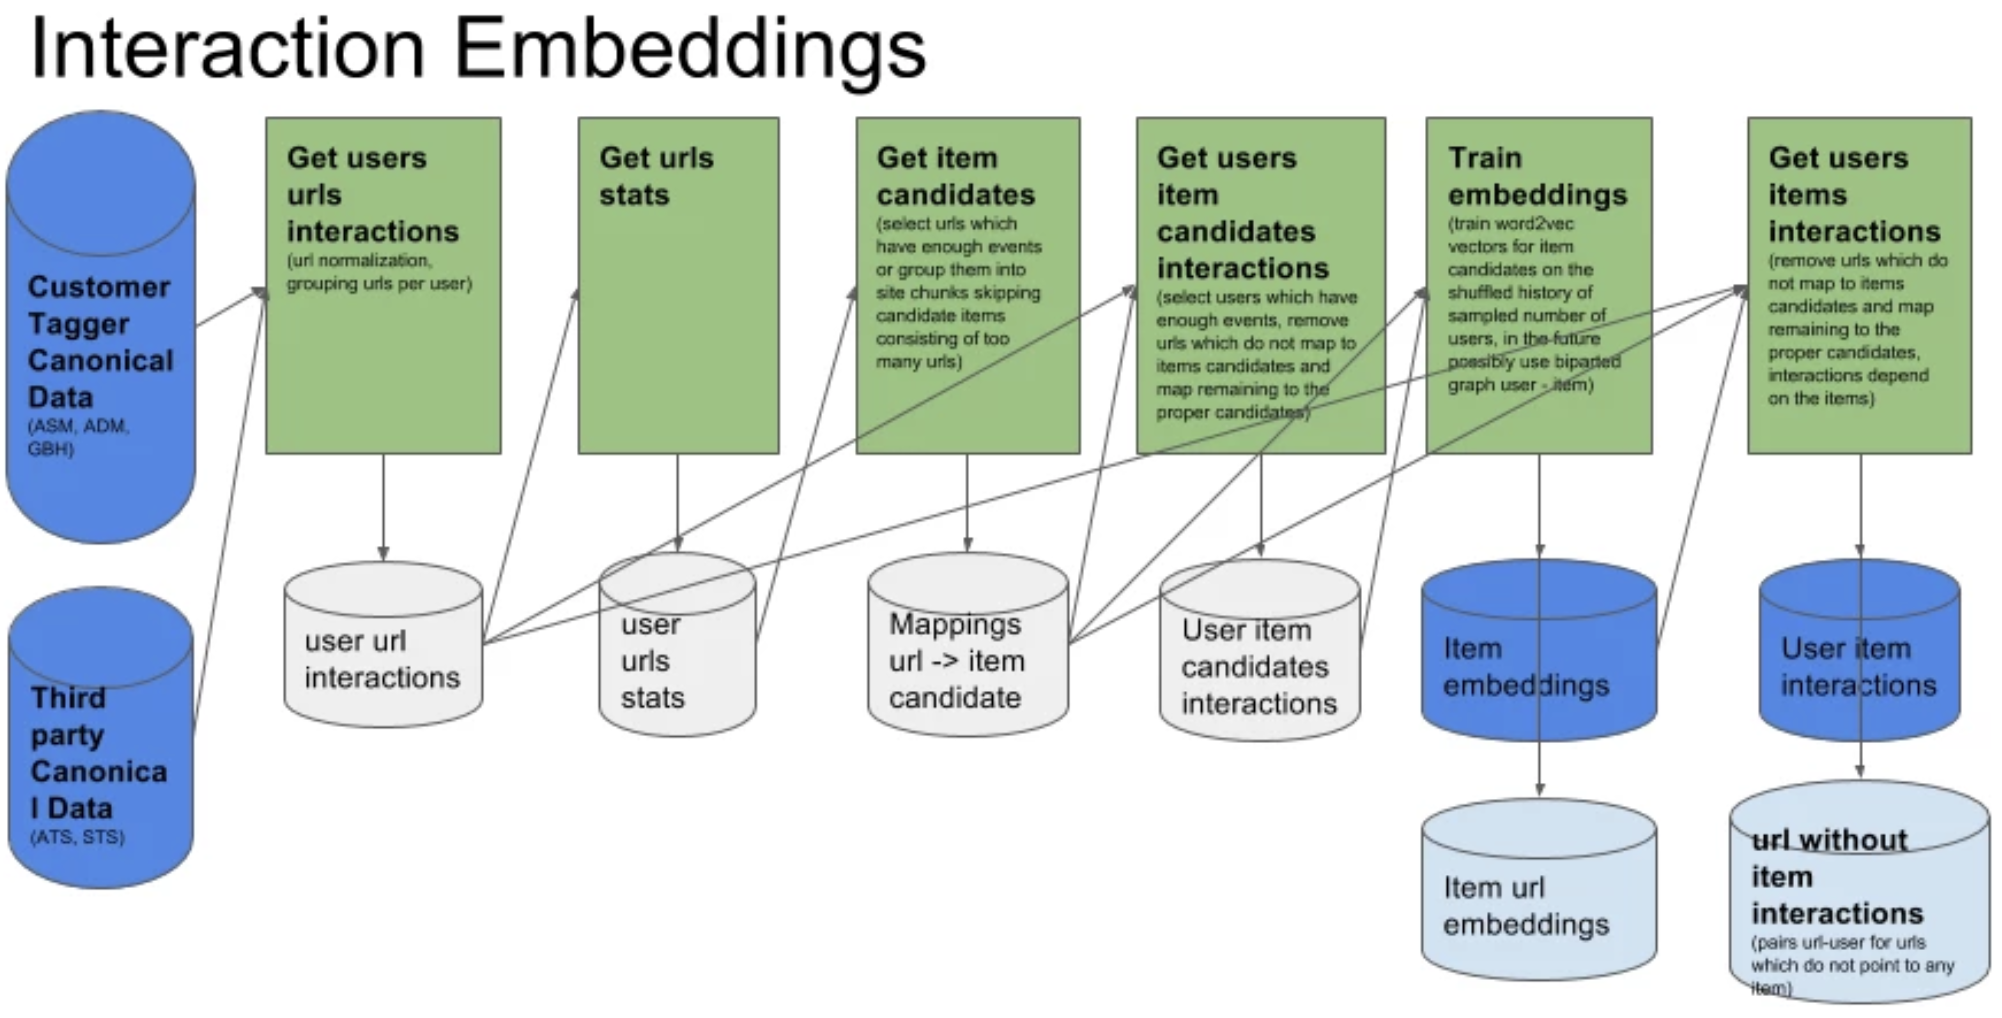
\includegraphics[width=1.0\textwidth]{interaction_embeddings}
\end{center}
\caption{Data architecture for computing item embeddings.}
\label{fig:architecture}
\end{figure}

The input to the ML subsystem for embeddings is thus the set of events per userID that has been seen in the last 60-90 days. The collection of items (URIs) per user is considered as a document that describes the user. And the collection of all the users is considered as a document collection. This allows us to treat the URIs as words in a language model and use results from deep representation learning techniques as applied to Natural Language Processing (NLP). Using these models, we are able to learn a robust representation (embeddings) of both items and users which satisfy various desirable properties such as a complementarity, supplementarity, and compositionality. 

The item embedding computation module returns item embedding vectors of a configurable pre-specified dimensionality. This module is built from components such as word2vec, Gensim or Tensorflow. This allows scaling-up to hundreds of thousands of items. In the event that there are more items, this can be handled via parallel execution of embedding computations (offered in Tensorflow for example) or by downsampling items accordingly by thresholding on frequency. 

\section{Milestone 4}

\subsection{Comparative Evaluation}

We have built major functionality into an existing Gensim implementation at 1plusX for learning embeddings for items and users. In the context of this project, we have also build from scratch a Tensorflow implementation of all machine learning models and algorithms, resulting in a more or less equivalent system. We have benchmarked different Gensim and different Tensorflow implementations to learn embeddings. The key metrics are summarized in Table \ref{tab:comp}.
\begin{table}
\begin{center}
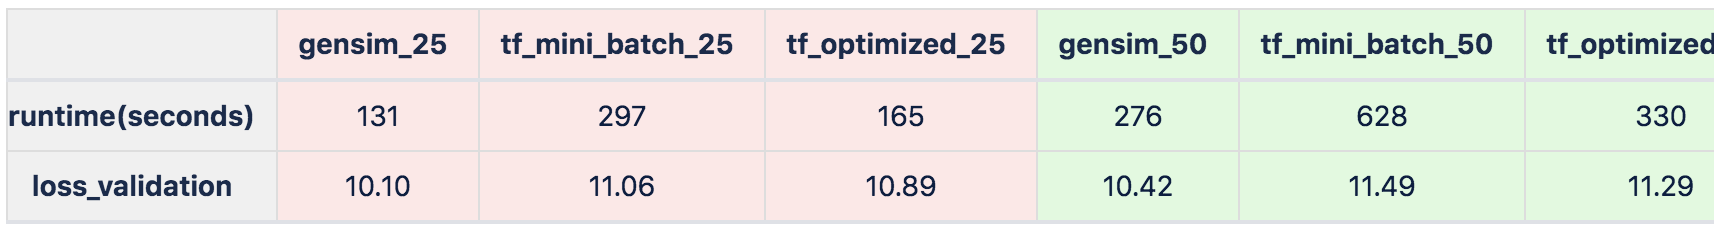
\includegraphics[width=\textwidth]{comp}
\end{center}
\caption{Comparison of performance and accuracy between models trained with Gensim and Tensorflow. For evaluation a standard internal data set of user-page visits has been used.}
\label{tab:comp}
\end{table}
One observes that Gensim has slight advantages in both, performance and final accuracy. However, the Tensorflow implementation comes close and has the advantage to be much more extensible as the framework is more powerful and flexible. We have drilled down a bit deeper and looked at different data set sizes (more ``words'' = visited URLs). Results in terms of accuracy and runtime are shown in Figure \ref{fig:comp}. \begin{figure}
\begin{center}
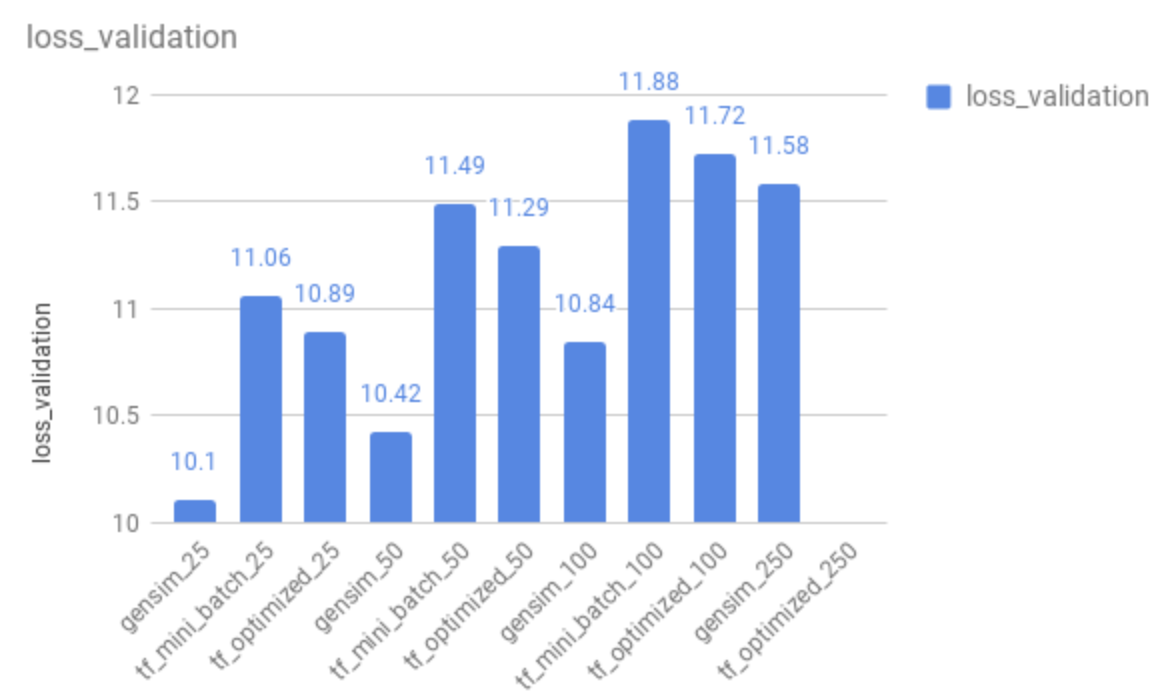
\includegraphics[width=0.48\textwidth]{loss_val}
\
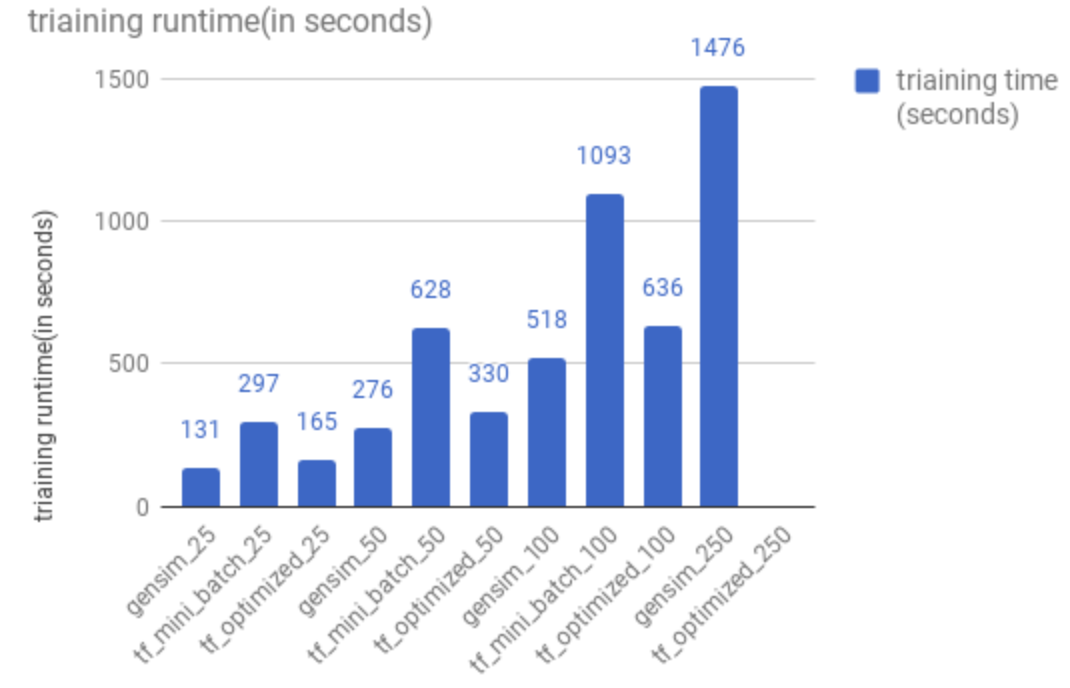
\includegraphics[width=0.48\textwidth]{run_val}
\end{center}
\caption{Comparison of accuracy/loss and runtime between models trained with Gensim and Tensorflow on different data set sizes.}
\label{fig:comp}
\end{figure}
Details on the data set preparation are shown in Table \ref{tab:data}. As one can see these data sets are quite big, ranging up to about 60M events. 
\begin{table}
\begin{center}
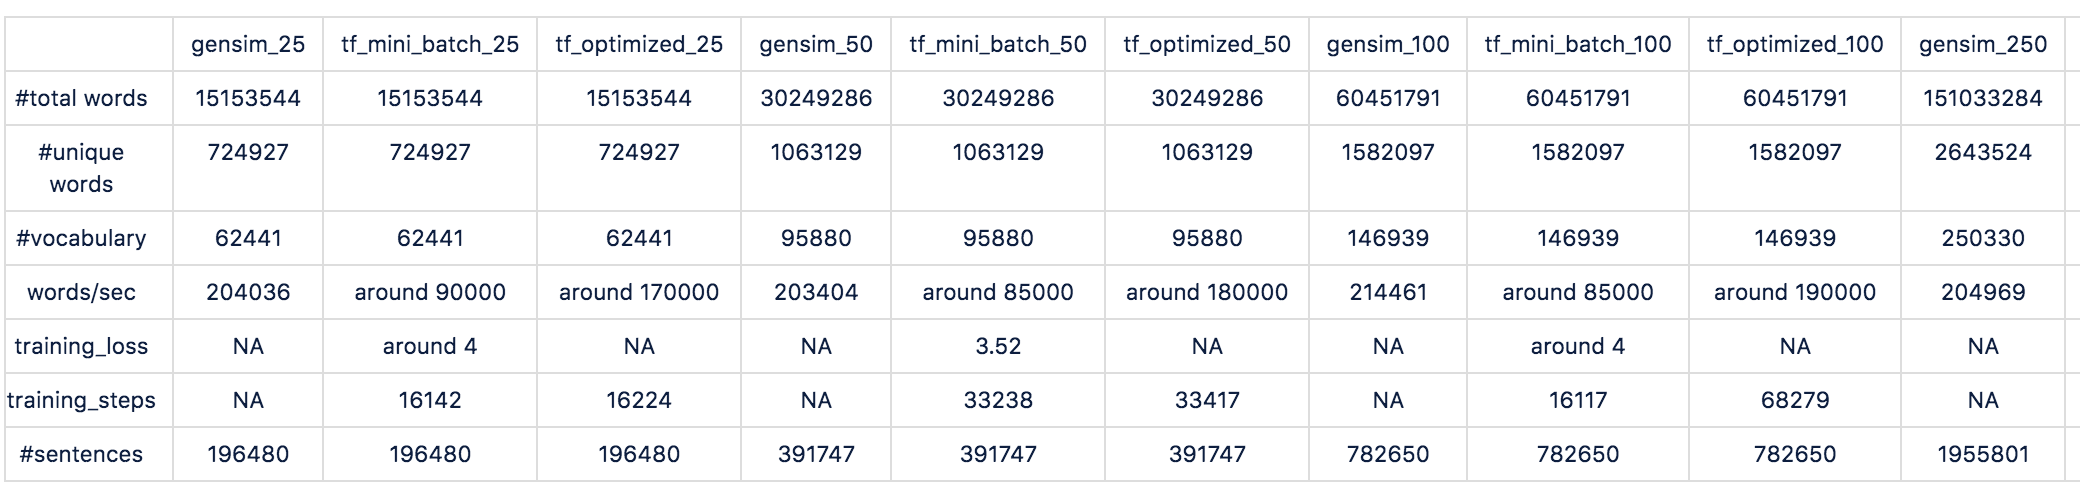
\includegraphics[width=\textwidth]{data_val}
\end{center}
\caption{Characteristics and dimensions of different data sets used in the experiments.}
\label{tab:data}
\end{table}

\subsection{Tensorflow Implementation}

We have built upon the Tensorflow programming environment shown in Figure \ref{fig:tensorflow}. In a first step, (1) we encapsulate the training data, which gets extracted from the logs in a form that is digestible for Tensorflow. Then one can use a simple jupyter notebook to (2) load pre-trained embedding models,  (3) train and evaluate pre-made tensorflow estimators (e.g.~classifiers) as a baseline, (4) build and train custom estimators with tf.keras, (4) export and deploy the models to the Google Cloud ML Engine, and (5) request inferences for single samples or for a batch from the cloud, using python or the command line.

This provides a powerful extension to 1plusX offering as it opens-up data and foundational models (i.e.~embeddings, pre-trained representations) to the Tensorflow ecosystem. The above pipeline has been tested and validated internally at 1plusX over various data sets from different existing customers.  The internal library is called TFplusX and a workflow demo can be found online at this \href{https://gist.github.com/Zacharias030/a56194322259ec336954ce4452aef68f}{public Github URL}.

\section{Milestone 5}

We have worked with an 1plusX customer, who does not come from the core segment of publishers and media resellers and who has a non-standard set of use cases and who needs custom models to be adapted to their needs.\footnote{The customer identity is not publicly known as hence can not be disclosed, but it is a large financial institution.} This customer was interested in age, gender, and interest prediction, audience expansion (finding users similar to a given core group), use of topic-based targeting, used two standard activation channels, and required custom events. 

We have pursued the approach outlined above and made processed data as well as embedding models and classifiers available as outlined above. The customer ran a pilot project in late 2018.  This pilot was deemed successful and the customer has continued towards productionizing the setup. It has not yet made use of the full Tensorflow capabilities due to legacy systems, but we expect the pilot customer as well as other customers to move in a direction that makes more use of the Tensorflow platform in the future (see also implementation plan).



\begin{figure}
\begin{center}
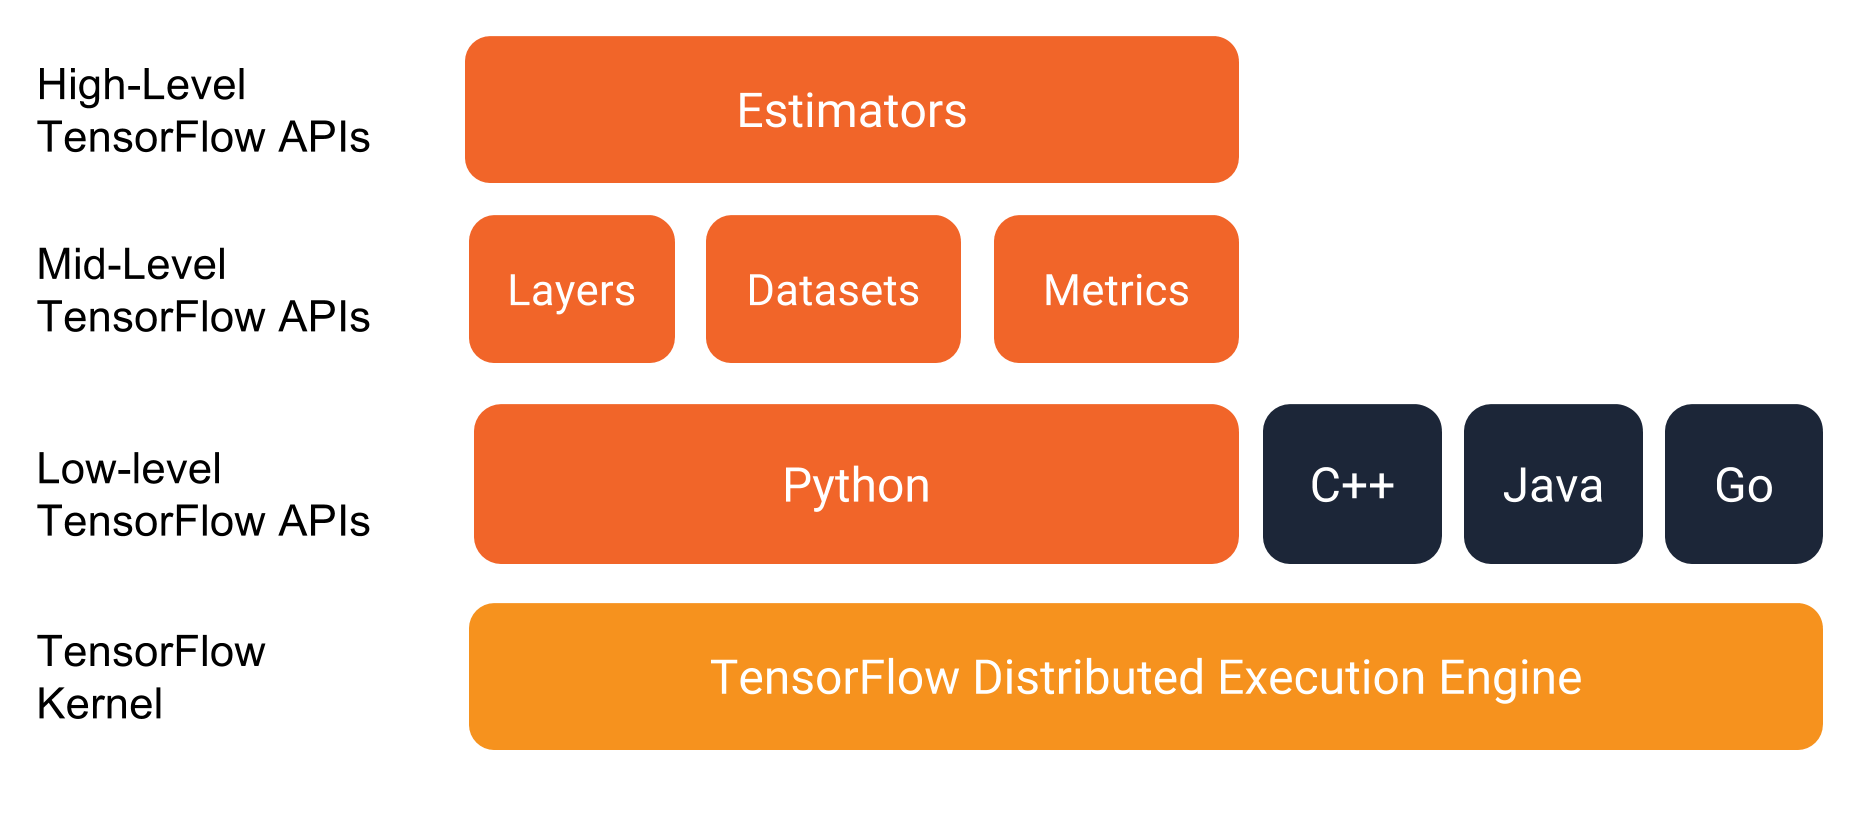
\includegraphics[width=\textwidth]{tensorflow_programming_environment}
\end{center}
\caption{Tensoflow programming environment}
\label{fig:tensorflow}
\end{figure}





\end{document}